\documentclass{article}
\usepackage[UTF8, heading = false, scheme = plain]{ctex}

\usepackage{geometry}
\geometry{b5paper,left=2cm,right=2cm,top=2cm,bottom=2cm}

\usepackage{color}
\usepackage{amsfonts}
\usepackage{amsmath}

\linespread{1.5}

\usepackage[colorlinks,
            linkcolor=red,
            anchorcolor=blue,
            citecolor=green
            ]{hyperref}

\usepackage{listings}
\usepackage{fontspec}
\newfontfamily\monaco{Monaco}
\definecolor{dkgreen}{rgb}{0,0.6,0}
\definecolor{gray}{rgb}{0.5,0.5,0.5}
\definecolor{mauve}{rgb}{0.58,0,0.82}
\lstset{ %
  basicstyle=\footnotesize\monaco,       % the size of the fonts that are used for the code
  numbers=left,                   % where to put the line-numbers
  numberstyle=\footnotesize\monaco\color{gray},  % the style that is used for the line-numbers
  numbersep=5pt
  stepnumber=1,                   % the step between two line-numbers. If it's 1, each line
                                  % will be numbered
  numbersep=5pt,                  % how far the line-numbers are from the code
  backgroundcolor=\color{white},      % choose the background color. You must add \usepackage{color}
  showspaces=false,               % show spaces adding particular underscores
  showstringspaces=false,         % underline spaces within strings
  showtabs=false,                 % show tabs within strings adding particular underscores
  frame=single,                   % adds a frame around the code
  rulecolor=\color{black},        % if not set, the frame-color may be changed on line-breaks within not-black text (e.g. commens (green here))
  tabsize=4,                      % sets default tabsize to 2 spaces
  captionpos=t,                   % sets the caption-position to bottom
  breaklines=true,                % sets automatic line breaking
  breakatwhitespace=false,        % sets if automatic breaks should only happen at whitespace
  title=\lstname,                   % show the filename of files included with \lstinputlisting;
                                  % also try caption instead of title
  keywordstyle=\color{blue},          % keyword style
  commentstyle=\color{dkgreen},       % comment style
  stringstyle=\color{mauve},         % string literal style
  escapeinside={\%*}{*)},            % if you want to add LaTeX within your code
  morekeywords={*,...}               % if you want to add more keywords to the set
}

\usepackage{amssymb} 

\setlength{\parindent}{2em}

\renewcommand{\G}{\mathbb{G}}
\newcommand{\Z}{\mathbb{Z}}
\newcommand{\Q}{\mathbb{Q}}
\newcommand{\F}{\mathbb{F}}

\newcommand{\Sbox}{\textsf{Sbox}}
\newcommand{\code}[1]{\lstinline!#1!}

%%%%%%%处理下划线:_%%%%%%%%%
\usepackage{underscore}
%%%%%%%处理下划线:_%%%%%%%%%

\setlength{\parindent}{2.1em}

\begin{document}

\title{ECDSA签名机制在区块链领域中的应用}
\author{longcpp \\ longcpp9@gmail.com}

\maketitle

\section{椭圆曲线secp256k1与secp256r1}

由于Bitcoin中的采纳,曾经未曾得到广泛部署的椭圆曲线secp256k1成为了大多数区块链项目中默认的椭圆曲线选择.
曲线secp256k1的名字来自于密码学标准文档SEC2~\cite{}~,其中``sec"是``Standards For Efficient Cryptography"缩写,
``p"表示椭圆曲线参数定义在有限域$\F_p$上, ``256"表示该有限域中元素的比特长度为256, 
``k"表示这是一条Koblitz曲线, 而``1"表示这是满足前述条件的第一条(实际上也是唯一的)推荐的曲线.
Koblitz曲线在密码学文献中通常指代定义在特征为2的有限域上$\F_{2^m}, m\in\Z$的椭圆曲线,
Gallant, Lamber和Vanstone1在CRYPTO 2001的论文\footnote{
Gallant, Robert P., Robert J. Lambert, and Scott A. Vanstone. "Faster point multiplication on elliptic curves with efficient endomorphisms." In Annual International Cryptology Conference, pp. 190-200. Springer, Berlin, Heidelberg, 2001.
\url{https://www.iacr.org/archive/crypto2001/21390189.pdf}}
中泛化了Koblitz曲线的含义,也包括定义在大素数上$\F_p$上具备高效可计算自同态特性的椭圆曲线.

Satoshi在最开始选择secp256k1曲线的原因仍不可知,尤其是在当时得到广泛部署的是一条名为secp256r1椭圆曲线的背景之下.
原因可能是secp256k1曲线具备的高效可计算的自同态映射可以加速ECDSA签名验证过程的特性在区块链场景中尤为合适,
但是以OpenSSL为代表的各个密码学库的实现中并没有利用这一属性.
虽然libsecp256k1中的实现成功利用这一属性使得基于secp256k1的ECDSA签名验证速度达到了21000次每秒
(测试平台的芯片型号为 Intel(R) Core(TM) i7-6700HQ CPU), 速度上超过了OpenSSL 1.1版本中深度优化的基于secp256r1曲线的
ECDSA的12000次每秒的验签速度,最终证实了secp256k1曲线在ECDSA验签操作中的效率优势,但是在选定这条曲线时,
并没有相应的实现可以证实关于验签效率的推断.

然而后来的斯诺登泄露的文档中显示的NSA可能在NIST标准中的埋藏算法级后门的信息,尤其经过Dual_EC_DRBG
事件\footnote{
Bernstein, D.J., Lange, T. and Niederhagen, R., 2016. Dual EC: A standardized back door. In The New Codebreakers (pp. 256-281). Springer, Berlin, Heidelberg.
\url{https://projectbullrun.org/dual-ec/documents/dual-ec-20150731.pdf}}
验证之后, Satoshi当初的曲线选择在后来看来有了先见之明的意味. 
得到广泛部署的secp256r1曲线中的``r"表示曲线参数是从随机种子派生而来. 
secp256r1 (NIST P-256)曲线的参数是从随机种子
$$c49d3608 86e70493 6a6678e1 139d26b7 819f7e90$$
中派生而来, 而该随机种子的来源NIST并没有解释,鉴于Dual_EC_DRBG事件的教训,难免会有其中存在后门的疑虑
\footnote{\url{http://safecurves.cr.yp.to/rigid.html}}.
相比之下, secp256k1曲线的参数选择有合理的解释,也就有助于消除对存在算法级后门的担忧
\footnote{\url{https://bitcointalk.org/index.php?topic=289795.msg3183975\#msg3183975}}.
后续介绍基于secp256k1的ECDSA签名机制在区块链领域中的应用以及在区块链场景下的面临的特殊问题.

\section{基于椭圆曲线secp256k1的ECDSA签名}

定义在有限域$\F_p$上的曲线secp256k1的方程为$y^2 = x^3 + 7$,其中
\footnotesize
$$p = 0xfffffffffffffffffffffffffffffffffffffffffffffffffffffffefffffc2f.$$
\normalsize
椭圆曲线上的点的个数为$\#E(\F_p) = h \cdot n$,其中$h = 1$为余因子(Cofactor), $n$为$E(\F_p)$的最大素子群的阶:
\footnotesize
$$ n = 0xfffffffffffffffffffffffffffffffebaaedce6af48a03bbfd25e8cd0364141.$$
\normalsize
子群 $\G = \langle G \rangle$的基点$G$的坐标为:
\footnotesize
$$G_x = 0x79be667ef9dcbbac55a06295ce870b07029bfcdb2dce28d959f2815b16f81798$$
$$G_y = 0x483ada7726a3c4655da4fbfc0e1108a8fd17b448a68554199c47d08ffb10d4b8$$
\normalsize
值得提及的是, $\G$的阶$n$是素数,也即$\F_n$是有限域,非零元构成的乘法群表示为$\F_n^*$.

假设待签名消息为$m$, 私钥为$d$, 公钥为$P=dG$, 哈希算法为$H: \{0,1\}^*\rightarrow\F_n^*$.
\textbf{ECDSA签名值$\sigma = (r,s), r, s \in \F_n^*$的计算过程}为: 
\begin{enumerate}
\item 选择随机数$k\in_R\F_n^*$, 计算$R = (x,y) = kG, x, y \in \F_p$, 计算$r = x\mod n \in \F_n^*$,
\item 计算消息$m$的哈希值$h=H(m)\in\F_n^*$, 计算 $s = k^{-1} (h + rd) \mod n$. 
\end{enumerate}
注意$k, r, s \in \F_n^*$,也即$k, r, s$均不得为0, 如果为0, 则重新选择$k$进行计算.

给定消息$m$, 公钥$P$, 签名值$\sigma = (r, s)$, \textbf{签名验证的过程}为:
\begin{enumerate}
\item  验证$r, s$确实是$\F_n^*$中的元素,也即$r, s \in [1, n-1]$, 否则签名值无效,
\item 计算哈希值$h=H(m)\in\F_n^*$,并计算$s\in\F_n^*$的逆$s^{-1}$,
\item  计算$R' = (x', y') = s^{-1}(hG + rP)$, 
\item 判断$R' \neq \mathcal{O}$,否则验签失败, 判断 $x' \mod n = r$, 相等则验签成功,否则验签失败.
\end{enumerate}
合法的签名能够验证通过是因为
$$R' = s^{-1}(hG + rP) = s^{-1}(hG + r(dG)) = s^{-1}(h+rd)G = kG = R.$$
上述基于曲线secp256k1的ECDSA签名机制,总共涉及3种数学结构上的计算:
有限域$\F_n$上加法和乘法运算(求逆运算可以由加法和乘法运算构造), $E(\F_p)$中的加法点群$\G$中点的加法运算(点的倍乘),
由于$\G$中的点的坐标为有限域$\F_p$中的元素,则点的加法运算中也涉及到有限域$\F_p$上的加法和乘法运算(求逆运算).
编码实现ECDSA签名机制时,需注意区分不同的运算,尤其要注意不要混淆有限域$\F_n$和$\F_p$上的运算.

\section{ECDSA签名机制应用中的安全隐患}

ECDSA签名机制在编码实现和应用时,特别是在区块链场景中应用时很容易引入安全问题,列举如下,随后依次介绍每个安全隐患的原理.
\begin{enumerate}
\item 如果$k$值泄露,则任何知道该随机数值的人可以使用该随机数产生签名值恢复私钥
\item 用相同私钥和$k$对两个消息进行签名,则任何人都可以通过两个签名值恢复出私钥
\item 两个用户使用相同的$k$分别对不同的消息进行签名,则任一方可推算出对方的私钥
\item 相同私钥和$k$同时用于ECDSA签名和Schnorr签名时,任何人都能够恢复出私钥
\item ECDSA签名值的可锻造性
\item 签名值通常采用的DER编码由于编码值并不唯一也会造成区块链网络的分裂
\item 不需要提供签名消息的情况下,任何人可以根据任意签名值伪造对应私钥的签名值
%\item 实现方面,侧信道攻击可以利用不安全的ECDSA签名实现窃取用于签名的私钥
\end{enumerate}

\subsection{随机数$k$值泄露导致私钥泄露}

签名过程中使用的随机数$k\in\F_n^*$一定要及时删除以免泄露.
这是因为知道随机数$k$的任何人,都可以根据签名值$\sigma=(r,s)$计算出相应的生成该签名值的私钥$d$.
随机数$k$的值与签名值$\sigma=(r,s)$之间的对应关系可以根据等式$x = (kG)_x \mod n = r$来进行判断.
由于$k$, $r$以及$h=H(m)$已知,则可以根据下面的公式计算私钥$d$:
$$s=k^{-1}(h+rd) \mod n \rightarrow ks = (h + rd)\mod n \rightarrow d = r^{-1}(ks - h)\mod n.$$

基于上述理由,在通过随机数发生器(Random Number Generator, RNG)生成随机数$k$的时候,
首先要确保选用的RNG生成的随机数的质量, 然后要确保生成的随机数没有被记录下来, 
还要确认RNG实现的安全性(生成$k$的能量消耗等侧信道信息不会泄露$k$的值),最后在使用完随机数$k$之后要将其及时删除.

\subsection{同一用户重用随机数$k$导致私钥泄露\label{subsec-1usereusek}}

如果同一个用户使用自己的私钥对不同的消息进行签名时,使用了相同的$k$值,则任何人可以根据消息和签名值推算出用户的私钥.
假设用户用私钥$d$和$k$对消息$m_1$和$m_2$进行签名,生成了签名值$\sigma_1=(r, s_1)$和$\sigma_2=(r, s_2)$,
可以看到两个签名值的$r$部分相同,这是因为使用了相同的$k$,而$r = (kG)_x \mod n$, 根据签名计算过程则有:
\begin{equation}\nonumber
\left\{
\begin{array}{lll}
s_1 = & k^{-1}(h_1 + rd) \mod n, & h_1 = H(m_1)\\
s_2 = & k^{-1}(h_2 + rd) \mod n, & h_2 = H(m_2)
\end{array}
\right.
\end{equation}
上面的方程组中,可以看到未知的变量仅有$k$和$d$,两个方程两个未知量,通过解方程组可以推算出私钥$d$.
根据上面的方程组就有
\begin{equation}\nonumber
\left\{
\begin{array}{ll}
k = & s_1^{-1} (h_1 + rd) \mod n \\
k = & s_2^{-1} (h_2 + rd) \mod n
\end{array}
\right.
\ 
\rightarrow
\ 
\dfrac{h_1+rd}{s_1^{-1}} = \dfrac{h_2+rd}{s_2^{-1}} \mod n
\end{equation}
根据$s_2(h_1+rd) = s_1(h_2+rd)\mod n$,可以推断出私钥
$$d = \dfrac{s_2h_1 - s_1h_2}{(s_1-s_2)r} \mod n.$$

\subsection{不同用户重用随机数$k$导致私钥泄露\label{subsec-2usereusek}}

前一小节论述了同一个用户签名时重用随机数$k$的安全隐患, 然而如果两个用户之间重用了随机数$k$, 同样也会私钥泄露的隐患.
如果两个用户Alice和Bob在用自己的私钥签名时,选用了同样的随机数$k$,
则Alice可以根据签名值推算出Bob的私钥, Bob也可以根据签名值推算出Alice的私钥.
假设Alice的私钥为$d_1$, 要签名的消息为$m_1$, 选用随机数$k$时计算的签名值为$\sigma_1 = (r, s_1)$,
Bob的私钥为$d_2$, 要签名的消息为$m_2$, 选用同样随机数$k$时计算的签名值为$\sigma_2 = (r, s_2)$.
则根据签名值的计算过程有
\begin{equation}\nonumber
\left\{
\begin{array}{lll}
s_1 = & k^{-1}(h_1 + rd_1) \mod n, & h_1 = H(m_1)\\
s_2 = & k^{-1}(h_2 + rd_2) \mod n, & h_2 = H(m_2)
\end{array}
\right.
\end{equation}
根据上面的方程组就有
\begin{equation}\nonumber
\left\{
\begin{array}{ll}
k = & s_1^{-1} (h_1 + rd_1) \mod n \\
k = & s_2^{-1} (h_2 + rd_2) \mod n
\end{array}
\right.
\ 
\rightarrow
\ 
\dfrac{h_1+rd_1}{s_1^{-1}} = \dfrac{h_2+rd_2}{s_2^{-1}} \mod n
\end{equation}
则有$s_2(h_1+rd_1) = s_1(h_2+rd_2) \mod n$.
在Alice看来,等式中未知的变量只有Bob的私钥$d_2$, Alice可以计算Bob私钥:
$$d_2 = \dfrac{s_2h_1 - s_1h_2 + s_2rd_1}{s_1r} \mod n,$$
而在Bob看来,等式中未知的变量只有Alice的私钥$d_1$, Bob可以计算Alice的私钥:
$$d_1 = \dfrac{s_1h_2 - s_2h_1 + s_1rd_2}{s_2r} \mod n.$$

Bitcoin历史上由于~\ref{subsec-1usereusek}~小节和~\ref{subsec-2usereusek}~小节中介绍的
关于随机数$k$的问题引发的多起私钥泄露的事件. 
由于安全的随机数发生器实现的困难性与程序员正确使用随机数的困难性,
业界由随机产生$k$逐渐切换为利用RFC 6979\footnote{
RFC 6979: Deterministic Usage of the Digital Signature Algorithm (DSA) and Elliptic Curve Digital Signature Algorithm (ECDSA).
\url{https://tools.ietf.org/html/rfc6979}}中推荐的方式.
RFC 6979中通过利用待签名消息$m$和私钥$d$等信息给出了一种确定性派生$k$的方式,
通过这种方式,只要$k$和$m$不同,在$k$值不同,也就避免了\ref{subsec-1usereusek}~小节和~\ref{subsec-2usereusek}~小节的安全隐患.

\subsection{ECDSA与Schnorr共用$k$导致私钥泄露\label{subsec-ecdsaschnorr}}

前面两个小节可以看到,同一用户重用$k$,不同用户重用$k$都会导致用于签名的私钥泄露的问题.
然而除了用户自己/用户之间重用$k$之外,如果不同的签名机制在签名时重用了$k$也同样会导致私钥泄露.
Bitcoin和Bitcoin Cash网络中正在围绕在链上采纳Schnorr签名而做大量的准备活动,
其中Bitcoin Cash已经在19年5月份的网络协议升级中为交易签名过程添加Schnorr签名机制.

首先介绍定义在椭圆曲线secp256k1上的Schnorr签名机制可以与ECDSA签名机制共用相同的公私钥对,
也即用于ECDSA签名的公私钥对$d\in\F_n^*, Q=dG\in\G$,同时也可以是Schnorr签名机制的公私钥对.
假设待签名消息为$m$,有哈希函数$H: \{0,1\}^*\rightarrow \F_n^*$, 
则\textbf{Schnorr签名$\sigma=(R,s), R\in \G, s\in\F_n^*$的计算过程}为:
\begin{enumerate}
\item 选取随机数$k\in_R\F_n^*$, 计算 $R=(x,y)=kG$,
\item 计算哈希值$h = H(R||P||m)\in\F_n^*$, 计算$s=r+hd \mod n \in \F_n^*$.
\end{enumerate}
给定消息$m$,公钥$P$, Schnorr签名值$\sigma=(R,s)$, \textbf{Schnorr签名验证过程}为:
\begin{enumerate}
\item 验证$R$确实是$\G$中的元素,验证$s$确实是$\F_n^*$中的元素,否则验签失败,
\item 计算哈希值$h = H(R||P||m)\in\F_n^*$,
\item 计算$R+hP$并验证是否与$sG$相等,如果相等验签通过,否则验签失败.
\end{enumerate}
合法的签名值能够验证通过是因为:
$$
sG = (k+hx)G = kG + hxG = R + h(dG) = R + hP.
$$
值得提及的是Schnorr签名还有另外一种变体,此处仅介绍Bitcoin和Bitcoin Cash网络中采用的Schnorr签名机制,
对于展示ECDSA和Schnorr签名共用$k$导致私钥泄露的问题来说已经足够.

用$d, P$表示ECDSA和Schnorr签名所共用的公私钥对, ECDSA签名用随机数$k$对消息$m_1$的签名值为$\sigma_1 = (r, s_1)$,
Schnorr签名用相同的随机数对消息$m_2$的签名值为$\sigma_2 = (R, s_2)$,下面展示如何通过签名值恢复私钥$d$.
根据签名计算规则有
\begin{equation}\nonumber
\left\{
\begin{array}{lll}
s_1 = & k^{-1}(h_1 + rd) \mod n, & h_1 = H(m_1)\\
s_2 = & k + h_2d \mod n, & h_2 = H(R||P||m_2)
\end{array}
\right.
\end{equation}
则有$k = s_2 - h_2d\mod n$,带入上述方程组的第一个等式得到
$$
s_1 =  (s_2 - h_2d)^{-1}(h_1 + rd) \mod n \rightarrow d = \dfrac{s_1s_2 - h_1}{s_1h_2 + r} \mod n.
$$

前面我们提到利用RFC 6979中的方法避开\ref{subsec-1usereusek}~小节和~\ref{subsec-2usereusek}~小节重用$k$的问题,
如何在不同的签名算法的维度上避免重用$k$? 答案是同样利用RFC 6979. 
RFC6979中输入参数可以包含``addition data", 在派生$k$时, 可以将签名算法的信息填入该字段, 如此可以在算法的维度上重用$k$.
可以参考Bitcoin Cash网络中支持Schnorr签名值的做法:

\textit{
We suggest using the RFC6979 sec 3.6 'additional data' mechanism, by appending the 16-byte ASCII string "Schnorr+SHA256␣␣" (here ␣ represents 0x20 -- ASCII space). The popular library libsecp256k1 supports passing a parameter \code{algo16} to \code{nonce_function_rfc6979} for this purpose.
}\footnote{\url{https://github.com/bitcoincashorg/bitcoincash.org/blob/master/spec/2019-05-15-schnorr.md}}

\subsection{ECDSA签名值的可锻造性问题\label{subsec-lowers}}

给定消息$m$的ECDSA签名值$\sigma=(r, s)$, 任何人都可以构造关于消息$m$的额外的合法签名值,
例如$\sigma'=(r, -s)$也是消息$m$的合法签名值, 也即$\sigma$和$\sigma'$均可利用公钥$P$验证通过.
这是因为验签是通过计算$R'=(x',y')=s^{-1}(hG + rP)$并判断$x' \mod n$是否等于签名值中的$r = x \mod n, (x, y) = R = kG$. 
然而根据椭圆曲线的性质有$-R' = (x', -y')$,也即$R'$和$-R'$具有相同的横坐标.
根据费马小定理有$s^{-1}\mod n \equiv s^{n-2} \mod n$以及有限域$\F_n$上$-s \equiv (n-s) \mod n$, 
根据多项式的二项展开(Binomial Expansion)有:
$$
\begin{array}{ll}
(-s)^{-1}\mod n & \equiv (n-s)^{n-2} \mod n \\
 & \equiv \sum_{i=0}^{n-2}\tbinom{n-2}{i}n^{n-2-i}(-s)^{i} \mod n \\
 & \equiv (-s)^{n-2} \mod n \\ 
 &  \equiv (-1)^{n-2}s^{-1}\mod n \\
 & \equiv -s^{-1}\mod n.
 \end{array}
$$
则验证签名值$\sigma'  = (r, -s)$时
$$
(-s)^{-1}(hG+rP) = -s^{-1}(hG + rP) = -R' = (x', -y'),
$$
由于$x' \mod n \equiv r \mod n$, 因此$\sigma'  = (r, -s)$验签成功.

两个签名值$\sigma=(r, s)$和$\sigma'  = (r, -s)$同时为消息$m$的合法签名,在很多场景中不会造成问题.
然而在区块链场景下,网络中的任何一方可以利用该性质,修改一笔交易中的签名值.
由于区块链中的交易ID通常是交易的哈希值,则ECDSA签名值的可锻造性会造成同一笔交易在网络上有不同的交易ID.
交易ID的不唯一会导致根据交易ID追踪交易状态时出现安全隐患.
假设追踪的是携带签名值$\sigma$的交易的ID,而上链的交易中包含的$\sigma'$ (具有不同的交易的ID),
则在数字货币交易所处理用户的提币操作时,当一笔提币已经成功时,根据交易ID进行交易状态跟踪的业务逻辑会认为提币操作失败.
倘若还设置了超时重试机制,会导致交易所资产的损失.

由于ECDSA签名值的可锻造性可能带来的安全隐患, BIP-146中针对ECDSA签名值做了额外的固定,
规定验签时签名值$(r,s)$中的$s$的值必须满足$0x1 \leq s \leq n/2$, 根据曲线secp256k1的参数有
\footnotesize
$$
n/2 = 0x7fffffffffffffffffffffffffffffff5d576e7357a4501ddfe92f46681b20a0.
$$
\normalsize
由于模运算的性质,当$s < n/2 \rightarrow (n-s) > n / 2$并且有$s = n/2 \rightarrow (n-s) = n/2$,
也即BIP-146中对$s$取值范围的限定,使得$\sigma = (r, s)$和$\sigma' = (r, -s)$中仅有一个为合法的签名值,
从而避开ECDSA签名值的可锻造性带来的安全隐患.

\subsection{ECDSA签名值DER编码的不唯一问题}

在用Go语言重新实现Bitcoin Cash协议的Copernicus项目时
\footnote{An alternative implementation of the Bitcoin Cash protocol, written in Golang. \url{https://github.com/copernet/copernicus}}
遇到了这样一个问题, Listing~\ref{lst-baddersig}~中的DER编码的ECDSA签名
用函数~\code{secp256k1_ecdsa_signature_parse_der}~解析时(来自libsecp256k1)失败,
但是用另外一个函数~\code{ecdsa_signature_parse_der_lax}~可以成功解析.

\begin{lstlisting}[language=c, caption = 解析失败的DER编码的ECDSA签名, label=lst-baddersig]
    const char *sig_der =
        "3046"
        "0221"
        "002e6f0e8b515b5f25e837592e5e8a834cbe3fabaf98973edf88b19502e0180c2d"
        "0221"
        "00d03cc64f35fb277fe1b69270b542aca5620394ed7b7fae7a3546934dd6fe4288";
\end{lstlisting}

函数~\code{secp256k1_ecdsa_signature_parse_der}~实现内部的逻辑关系在Figure~\ref{fig-parsesig}中展示.
跟踪函数执行过程,可以发现错误发生在对函数~\code{secp256k1_ecdsa_sig_parse}~的调用,
更具体的说是该函数中调用~\code{secp256k1_der_parse_integer}~函数尝试对签名值的$r$解析时返回0值(执行失败).

\begin{figure}[h]
\centering
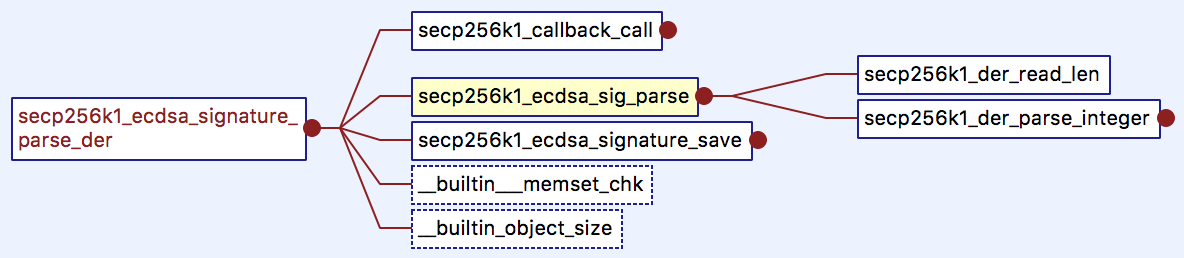
\includegraphics[width=\textwidth]{./secp256k1-ecdsa-signature-parse-der.png}
\caption{函数~\code{secp256k1_ecdsa_signature_parse_der}~内部实现逻辑}\label{fig-parsesig}
\end{figure}

继续追踪~\code{secp256k1_der_parse_integer}~的内部实现,可以发现导致失败的原因是上述签名值中表示$r$的部分
在最开始的多余额全零字节$00$, 对应函数内部的代码注释: \code{/* Excessive 0x00 padding. */}.
如下面代码展示,删掉多余的全零字节,并相应调整DER编码中指示长度的字段,则可用函数~\code{secp256k1_ecdsa_signature_parse_der}
成功解析签名值.

\begin{lstlisting}[language=c, caption = 可成功解析的DER编码的ECDSA签名, label=lst-gooddersig]
    const char *sig_der =
        "3045"
        "0220"
        "2e6f0e8b515b5f25e837592e5e8a834cbe3fabaf98973edf88b19502e0180c2d"
        "0221"
        "00d03cc64f35fb277fe1b69270b542aca5620394ed7b7fae7a3546934dd6fe4288";
\end{lstlisting}

为了明白上述问题的产生原因,接下来介绍DER (Distinguished Encoding Rules)编码规则,
DER编码是ASN.1 (Abstract Syntax Notation One)编码中的一种编码规则. 
ASN.1中另外支持的编码规则包括BER (Basic Encoding Rules)和CER( Canonical Encoding Rules).
其中DER和CER编码规则完全指定了编码规则,也即对于特定的数据仅有一个编码值是合法的.
DER针对数据长度的不同,有两种方式来编码数据载荷的长度: Short Encoding和Long Encoding, 
并规定当数据载荷的长度小于128个字节时,应当使用Short Encoding. 
基于secp256k1曲线的ECDSA签名值中的$r, s$都是256比特的整数,所以采用的是Short Encoding的DER编码方式.

Bitcoin中从OpenSSL中继承了签名值的DER编码方式,这是因为早期的Bitcoin的密码能力通过OpenSSL实现,
而OpenSSL中ECDSA签名操作的返回的是使用DER编码后的签名值.
由于签名值中的$r,s$都是证书,接下来仅考虑对INTEGER的编码方式.
对INTEGER的编码基本上是以字节为基本单位将整数表达成256进制表示,
编码规则同时要求对于正数($r,s$是正数),第一个字节的最高位必须为0,
如果第一个字节的最高位为1, 则需要在第一个字节之前添加一个全零字节.
另外DER编码规则同时规定,对于所有可能的编码值中,选用最短的编码值作为合法的签名值:

\textit{
The Distinguished Encoding Rules specify we must choose the shortest encoding that fully represents the length of the element.The encoded lengths do not include the ASN.1 header or length bytes, simply the payload.
}\footnote{
摘录自St Denis, Tom. Cryptography for developers. Elsevier, 2006.}

理论或者设想总是美好的,但是在具体实现时经常出现偏离规则的情况,正如OpenSSL的实现中DER解码时候
也会接受没有严格遵循前述规则的DER编码:

\textit{
One specifically critical area is the encoding of signatures. Until recently, OpenSSL's releases would accept various deviations from the DER standard and accept signatures as valid. When this changed in OpenSSL 1.0.0p and 1.0.1k, it made some nodes reject the chain.
}\footnote{
摘录自Wuille, Pieter. BIP-66: Strict DER signatures. 2015. \url{https://github.com/bitcoin/bips/blob/master/bip-0066.mediawiki}
}

在区块链场景中会引发的问题,如果各个节点运行的OpenSSL版本不同,则对于一个没有遵循DER规则的签名值编码,
可能会出现某些节点认为包含了这样签名的区块为合法区块,而另一些节点则将该节点视为非法的区块,从而导致网络的分裂.
因此, Bitcoin中在BIP-66中对Bitcoin网络应该接收的签名的DER编码做了更为严格的限制.

另外的问题在于, 签名值的DER编码在区块链的场景中是否是必要的? ECDSA签名值的DER编码长度根据具体的签名值,
长度会有所不同, 按照BIP-66中的约束,编码之后的签名值最多可以为73个字节, 相比之下直接采用$r, s$的二进制表示的话,
签名值则是固定的64个字节. 也因此,在Bitcoin和Bitcoin Cash计划中的采用Schnorr签名的升级,没有采用DER形式编码Schnorr签名值,
而是直接采用签名值的固定64个字节的二进制表示形式\footnote{
\textit{``Signature encoding: Instead of DER-encoding for signatures (which are variable size, and up to 72 bytes), we can use a simple fixed 64-byte format."} 
摘录自Wuille, Pieter. BIP-draft: Schnorr Signatures for secp256k1. 2018. 
\url{https://github.com/sipa/bips/blob/bip-schnorr/bip-schnorr.mediawiki}
}.

在Section~\ref{subsec-ecdsaschnorr}~中, 提到了Bitcoin和Bitcoin Cash采用的Schnor签名机制的签名值为$(R,s), R\in \G, s\in \F_n^*$.
注意到签名值中$R$是一个点, 而$s$是32字节的整数. 如何利用32个字节表达椭圆曲线上的一个点$R$? 
由于公钥$P$也是一个椭圆曲线上的一个点,不压缩形式的需要占用65个字节,而目前的公钥的压缩表示需要占用$33$个字节,
32个字节表示点的横坐标,另外一个字节指示点的纵坐标的取值(如果$(x, y)$满足$y^2=x^3 + 7$, 则$(x, -y)$也满足).
可是如何用32个字节表达椭圆曲线上的一个点? 可以看到, 33个字节的压缩形式的公钥表示是为了表达1比特的信息: $y$还是$-y$.
如果通过椭圆曲线的某种性质,对点的纵坐标取值进行限定,使得两种可能的纵坐标中仅有一个能够满足条件,则可以用32个字节表示点.
可以借鉴Section~\ref{subsec-lowers}~中通过限制取值范围来处理ECDSA签名值中可锻造性问题的方案, 
限制纵坐标的取值必须$\leq p/2$或者限制纵坐标的取值必须为奇数(或者必须为偶数). 
限制奇数或者偶数的原因在于$p$为奇数,则$y \mod p$和$-y \mod p$必然一个为奇数一个为偶数.
另外也可以通过约定$y$必须为是$\F_p$上的二次剩余(Quadratic Residue)的方式添加限制.
Pieter的关于Schnorr签名的BIP草稿``Schnorr Signatures for secp256k1"中采用的是通过二次剩余的方式添加对$y$值的约束.
选取的原因涉及椭圆曲线的实现细节(如Jacobi符号)以及效率因素,将在另外的文档再具体介绍.

\subsection{不需要提供签名值对应的消息$m$时可伪造签名值}

ECDSA签名过程中, 首先利用哈希函数对待签名消息$m$计算散列值, 然后针对散列值进行后续的计算.
验签操作也同样先对消息$m$进行哈希,并利用哈希值执行后续的验证操作.
然而一个较少提及的应用注意事项是, 验证签名时一定要提供消息$m$本身,而不能仅提供消息$m$的哈希值.
假设$\sigma=(r, s)$是使用私钥$d$对消息$m$计算的签名值,如果验签时不要求提供消息$m$本身(仅提供消息的哈希值$h$),
则任何人都可以伪造关于私钥$d$的签名值$\sigma'=(r', s')$.

根据ECDSA签名验证过程,验证一个利用私钥$d$对消息$m$签署的签名值$(r,s)$时,需要验证的条件为:
$$s^{-1}(hG+rP) = (x', y') = R', \  x' \mod n \equiv r, \text{ 其中 }\  r \equiv x \mod n, (x,y) = R = kG.$$

任何人都可以根据一个已知的合法签名值$\sigma=(r,s)$利用上式直接构建满足上式的$r', s'$,而无需知道私钥$d$.
构建时首先选择随机数$u, v\in_R\F_n^*$并计算$R' = (x', y') = uG + vP$, 令$r' \equiv x' \mod n$.
为了使最终的签名$\sigma' = (r', s')$在验签时,能够验证通过,需要$s'^{-1}(h'G  + r'P) = uG + vP$,则有
\begin{equation}\nonumber
\left\{
\begin{array}{ll}
s'^{-1}h' & \equiv u \mod n\\
s'^{-1}r' & \equiv v \mod n,
\end{array}
\right.
\rightarrow
\left\{
\begin{array}{ll}
s' & \equiv r'v^{-1} \mod n\\
h' & \equiv r'uv^{-1} \mod n
\end{array}
\right.
\end{equation}
则$\sigma = (r', s')$和哈希值$h'$利用公钥$Q=dG$也能够验证通过:
$$
s'^{-1}(h'G + r'P) = s'^{-1}h' G + s'^{-1}r'P = (r'^{-1}v r'uv^{-1})G + r'^{-1}vr' P  = uG + vP.
$$

如果在验证ECDSA签名时,要求提供哈希值所对应的消息$m$,则无法执行上述伪造签名的过程.
这是由于哈希函数的抗碰撞特性保证了从$h'$推导$m'$并且满足$h'=H(m')$是不可能的.
尝试先选定消息$m'\ \text{s.t.}\ h' = H(m')$来伪造签名也是不可能行, 因为为了成功构造签名$(r', s')$, 则需要
\begin{equation}\nonumber
\left\{
\begin{array}{ll}
s'^{-1}h' & \equiv u \mod n\\
s'^{-1}r' & \equiv v \mod n,
\end{array}
\right.
\rightarrow
h'u^{-1} \equiv s' \equiv r'v^{-1} \mod n
\rightarrow
r' \equiv h'u^{-1}v \mod n
\end{equation}
选择$u,v$的值,使得下面的方程组成立是不现实的.
\begin{equation}\nonumber
\left\{
\begin{array}{ll}
r' = & h'u^{-1}v \mod n\\
r ' = & x' \mod n,  (x', y') = uG + vP
\end{array}
\right.
\end{equation}
这是因为上述方程组等价于要求相同的$u,v$值按照不同的计算路径有相同的输出结果.
如果将两个不同的计算路径看做伪随机函数,则上述方程组等价于要求$2^{256}$空间上的两次相互独立的随机取值相同(碰撞).
根据生日悖论的结论,构建这样的碰撞大概需要$2^{128}$次操作,这是不现实的,
也即尝试通过先选定消息$m'\ \text{s.t.}\ h' = H(m')$来伪造签名是不可能行的.

Craig Wright (澳本聪)曾经利用本节介绍的原理通过伪造Satoshi Nakamoto的签名值,进而宣传自己为中本聪.
其实任何人都可以做类似的宣称,甚至有网站\footnote{
Prove to the world you are Satoshi Nakamoto. \url{https://albacore.io/faketoshi}}
提供了自动化的工具来帮助你宣称自己是中本聪.

\section{从ECDSA签名值逆推公钥}

尽量减少每一笔交易/每一个区块的大小,对于缩减区块体积, 提升区块的传播速度等方面大有裨益.
Bitcoin网络中一个典型的P2PKH交易的主要内容在Figure~\ref{fig-bitcoin-p2phk}~中展示
其中解锁脚本(Unlocking Script)中签名值\textsf{sig}按照DER编码长度大约为70个字节, 
压缩的公钥\textsf{PubK}需要33个字节(推荐使用压缩形式),
锁定脚本(Locking Script)中字节码\textsf{DUP}, \textsf{HASH160}, \textsf{EQUALVERIFY}, \textsf{CHECKSIG}各占用一个字节, 
而\textsf{PubKhash}为20个字节, 则Figure~\ref{fig-bitcoin-p2phk}~展示的脚本占用的链上存储空间大约为130个字节.

\begin{figure}[h]
\centering
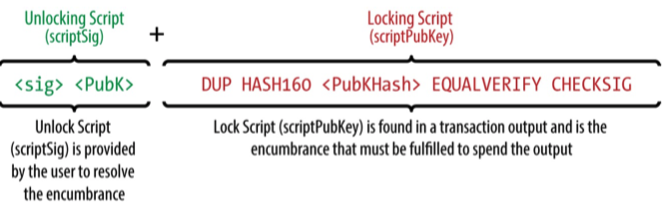
\includegraphics[width=\textwidth]{./bitcoin-p2pkh.png}
\caption{Bitcoin中的P2PKH交易: 解锁脚本与锁定脚本}\label{fig-bitcoin-p2phk}
\end{figure}

ECDSA签名机制的一个在区块链场景中非常有用但是Bitcoin中没有利用的特性是可以根据签名值\textsf{sig}推算出公钥\textsf{PubK},
下文中用可恢复签名来指代这一特性.
这意味着解锁脚本中的33个字节的压缩公钥\textsf{PubK}字段是冗余的.
利用从ECDSA签名值可以恢复公钥的特性, 解锁脚本中不再需要字段\textsf{PubK},
则Figure~\ref{fig-bitcoin-p2phk}~所示的交易只需要占用100个字节左右的存储空间,大约为23\%的存储空间节省.
如果Bitcoin从最开始就利用了这一特性,则同样大小的区块中可以存放更多交易,历史区块占用的存储空间也可得到大幅缩减.
Ethereum项目中利用了ECDSA签名机制的这一特性, Ethereum交易中没有包含公钥信息, 验签时从签名值推算即可.

实际上, 为了能够从签名值恢复出唯一的公钥值,还需要存储额外的信息,
也因此为了支持可恢复签名的特性, libsecp256k1库中定义了如Listing~\ref{lst-libsecp256k1-rsig}~中所示的可恢复签名结构体,
 根据注释可以看到该结构体的大小为65个字节.

\begin{lstlisting}[language=c, caption = libsecp256k1中的\textsf{secp256k1_ecdsa_recoverable_signature}, label=lst-libsecp256k1-rsig]
/** Opaque data structured that holds a parsed ECDSA signature,
 *  supporting pubkey recovery.
 *
 *  The exact representation of data inside is implementation defined and not
 *  guaranteed to be portable between different platforms or versions. It is
 *  however guaranteed to be 65 bytes in size, and can be safely copied/moved.
 *  If you need to convert to a format suitable for storage or transmission, use
 *  the secp256k1_ecdsa_signature_serialize_* and
 *  secp256k1_ecdsa_signature_parse_* functions.
 *
 *  Furthermore, it is guaranteed that identical signatures (including their
 *  recoverability) will have identical representation, so they can be
 *  memcmp'ed.
 */
typedef struct {
    unsigned char data[65];
} secp256k1_ecdsa_recoverable_signature;
\end{lstlisting}

对比Listing~\ref{lst-libsecp256k1-sig}中libsecp256k1中的普通ECDSA签名值(根据注释大小保证为64个字节),
可以注意到~\code{secp256k1_ecdsa_recoverable_signature}~需要额外的一个字节来存储额外的信息.
libsecp256k1也提供了相应的签名接口~\code{secp256k1_ecdsa_sign_recoverable}.

\begin{lstlisting}[language=c, caption = libsecp256k1中的\textsf{secp256k1_ecdsa_signature}, label=lst-libsecp256k1-sig]
/** Opaque data structured that holds a parsed ECDSA signature.
 *
 *  The exact representation of data inside is implementation defined and not
 *  guaranteed to be portable between different platforms or versions. It is
 *  however guaranteed to be 64 bytes in size, and can be safely copied/moved.
 *  If you need to convert to a format suitable for storage, transmission, or
 *  comparison, use the secp256k1_ecdsa_signature_serialize_* and
 *  secp256k1_ecdsa_signature_parse_* functions.
 */
typedef struct {
    unsigned char data[64];
} secp256k1_ecdsa_signature;
\end{lstlisting}

接下来介绍可恢复签名的原理,以及可恢复签名结构体中额外的一个字节中存储的信息和必要性.
首先关注ECDSA签名值中的$r \equiv x \mod n, (x, y) = kG, x, y \in \F_p$, 根据曲线secp256k1的参数可知,
$n < p < 2n$, 则当$x < n$时, $r = x$, 而当$x >= n$, 有$r = x + n$. 
也即根据$r$以及$x$是否大于$n$这1比特的信息可以唯一$R = kG$的横坐标$x$.
进一步根据椭圆曲线的方程可以从$x$的值计算出纵坐标$y$的值,前述已经论述过$y$和$-y$都是对应$x$的合法值,
也即根据$x$的值以及$y$为奇数还是偶数这1比特信息可以唯一确定点$R = kG$.
有了$R$信息之后,对于合法的签名可以通过如下推算公钥$P$:
$$
R = s^{-1}(hG+rP) \rightarrow rP = sR - hG \rightarrow P = r^{-1}(sR-hG).
$$


\begin{lstlisting}[language=c, caption = libsecp256k1中的\textsf{secp256k1_ecdsa_sig_sign}, label=lst-libsecp256k1-signimpl]
static int secp256k1_ecdsa_sig_sign(const secp256k1_ecmult_gen_context *ctx, secp256k1_scalar *sigr, secp256k1_scalar *sigs, const secp256k1_scalar *seckey, const secp256k1_scalar *message, const secp256k1_scalar *nonce, int *recid) {
    unsigned char b[32];
    secp256k1_gej rp;
    secp256k1_ge r;
    secp256k1_scalar n;
    int overflow = 0;

    secp256k1_ecmult_gen(ctx, &rp, nonce);
    secp256k1_ge_set_gej(&r, &rp);
    secp256k1_fe_normalize(&r.x);
    secp256k1_fe_normalize(&r.y);
    secp256k1_fe_get_b32(b, &r.x);
    secp256k1_scalar_set_b32(sigr, b, &overflow);
    /* These two conditions should be checked before calling */
    VERIFY_CHECK(!secp256k1_scalar_is_zero(sigr));
    VERIFY_CHECK(overflow == 0);

    if (recid) {
        /* The overflow condition is cryptographically unreachable as hitting it requires finding the discrete log
         * of some P where P.x >= order, and only 1 in about 2^127 points meet this criteria.
         */
        *recid = (overflow ? 2 : 0) | (secp256k1_fe_is_odd(&r.y) ? 1 : 0);
    }
    secp256k1_scalar_mul(&n, sigr, seckey);
    secp256k1_scalar_add(&n, &n, message);
    secp256k1_scalar_inverse(sigs, nonce);
    secp256k1_scalar_mul(sigs, sigs, &n);
    secp256k1_scalar_clear(&n);
    secp256k1_gej_clear(&rp);
    secp256k1_ge_clear(&r);
    if (secp256k1_scalar_is_zero(sigs)) {
        return 0;
    }
    if (secp256k1_scalar_is_high(sigs)) {
        secp256k1_scalar_negate(sigs, sigs);
        if (recid) {
            *recid ^= 1;
        }
    }
    return 1;
}
\end{lstlisting}


有了上述理论,可以通过libsecp256k1中函数~\code{secp256k1_ecdsa_sig_sign}~的实现来理解额外的一个字节中存储的信息,
参见Listing~\ref{lst-libsecp256k1-signimpl}.
函数参数~\code{recid}~对应可恢复签名结构体~\code{secp256k1_ecdsa_recoverable_signature}~中字节数组的最后一个字节.
根据第22行可知, 如果~\code{recid}~第2最低比特为1,表示$r > n$, 如果最低比特比特为1,则$R$的纵坐标是奇数.

\end{document}